% how to compile: pdflatex Template.tex. This will create a Template.pdf file.
\documentclass[11pt,fleqn]{article}
\usepackage{cite}
\usepackage{microtype}                  % improved microtypography
\usepackage[utf8]{inputenc}             % utf8 encoding
\usepackage{newtxtext}
\usepackage{newtxmath} 
\gdef\ttdefault{cmtt}%                                       
\usepackage{graphicx}                   % graphics
\usepackage{xcolor}                     % colors
\usepackage{amsmath}                    % ams math commands
\usepackage[margin=3cm]{geometry}       % page layout
\usepackage[english]{babel}             % english typographic rules
\usepackage{listings,xcolor}
\usepackage{booktabs}

%----------------------------------------------
% title page
\title{FEM Solver with Matlab}
\author{John Lian, Orginally written in April 2015}

%-------------------------------------------
\begin{document}
\maketitle                              % creates title page

\section{The exercise}

This document was part of a homework assignment originally submitted for MECH 546 - Finite Element Methods in Solid Mechanics at McGill University. 
The aim of the exercise was to build the stiffness matrix of the system depicted in Figure \ref{fig:exercise}. The mesh was to be generated using FreeFem++ and imported into Matlab using the linear triangular T3 finite  elements and assuming plane strains and a standard steel. The external force stems from (1) the vertical gravity with $g$ = 1000 m/s\textsuperscript{2} and (2) a constant pressure $P = 10^4$ N/m\textsuperscript{2}.

\begin{figure}[!h]
    \centering
    \includegraphics{exercise.png}
    \caption{System of interest. Distances are expressed in meters}
    \label{fig:exercise}
\end{figure}

\section{The solver and the methods} 

The system depicted was meshed in FreeFem++ with, essentially, a difference between a circle and an ellipse with a cut-off on the right. The circle has a radius of $R = 13$ and the ellipse is given by 

\begin{equation}
	\left(\frac{x-12}{12}\right)^2 + \frac{y^2}{5^2} = 1,
\end{equation}

thus, the ellipse is described with $a = 12$ and $b = 5$. The mesh was implemented in FreeFem++ using 

\begin{verbatim}
border aa(t=0,2*sqrt(R^2-9^2)){x=-9;y=ya-t;label=1;};
border bb(t=0,21){x=-9+t;y=-1*sqrt(R^2-x^2);label=2;};
border cc(t=0,12){x=12-t;y=-b*sqrt(1-(t/a)^2);label=3;};
border dd(t=0,12){x=t;y=b*sqrt(1-((t-12)/a)^2);label=4;};
border ee(t=0,21){x=12-t;y=sqrt(R^2-x^2);label=5;};
\end{verbatim}

A FEM solver was then implemented in MATLAB. In order to make the implementation more efficient (fewer for loops), some \emph{tricks} were employed. To begin, let $[T^e]$ be the triangle geometric matrix defined as 

\begin{equation}
	[T^e] = 
\left[
\begin{array}{ccc}
1 & 1 & 1 \\
x^e_1 & x^e_2 & x^e_3 \\
y^e_1 & y^e_2 & y^e_3
\end{array}
\right].
\end{equation}

Thus, the area of the triangle is given as $|T^e|$. With that, the elemental stiffness matrix is given as

\begin{equation}
	[K^e] = \dfrac{1}{4|T^e|}[B]^T[D][B]
\end{equation}

for a T3 element. It can be computed simultaneously for all indices using the fact that

\begin{equation}
\left[
\begin{array}{cc}
\frac{\partial N_1^{4Q}}{\partial x} & \frac{\partial N_1^{4Q}}{\partial y} \\
\frac{\partial N_2^{4Q}}{\partial x} & \frac{\partial N_2^{4Q}}{\partial y} \\
\frac{\partial N_3^{4Q}}{\partial x} & \frac{\partial N_3^{4Q}}{\partial y}
\end{array}
\right]
=
\left[
\begin{array}{ccc}
1 & 1 & 1 \\
x^e_1 & x^e_2 & x^e_3 \\
y^e_1 & y^e_2 & y^e_3
\end{array}
\right]^{-1}
\left[
\begin{array}{cc}
0 & 0 \\
1 & 0 \\
0 & 1
\end{array}
\right]
= \frac{1}{2|T^e|}
\left[
\begin{array}{ccc}
y_2^e-y_3^e & x_3^e-x_2^e \\
y_3^e-y_1^e & x_1^e-x_3^e \\
y_1^e-y_2^e & x_2^e-x_1^e
\end{array}
\right]
\end{equation}

Then, the assembly operation for the global stiffness matrix is given by

\begin{equation}
	[K_{ij}] = \sum_{T \in \Omega} [K^e_{ij}],
\end{equation}

where $T$ denotes T3 elements. 

Using similar logic, the force vector is given by

\begin{equation}
	(F_i) = \sum_{T \in \Omega} (F_{\Omega i}^e) + \sum_{E \in \partial\Omega} (F_{\partial \Omega i}^e),
\end{equation}

where $E$ are edges of the domain. 

Assuming body forces $f_{\Omega} = (f_1, f_2)$ are given at the mesh nodes, the integral can be approximated by 

\begin{equation}
\int_\Omega [N^e]^T f_{\Omega} d\Omega = \frac{1}{6} 
\left|
\begin{array}{ccc}
x_2^e - x_1^e & x_3^e - x_1^e \\
y_2^e - y_1^e & y_3^e - y_1^e
\end{array}
\right|
f_i(x_c,y_c), \quad j=\mod(i-1,2)+1
\end{equation}

where $(x_c,y_c)$ is the centre of mass of the triangle $T$. With the assumption on $f$,

\begin{equation}
	f_j(x_s, y_s) = (f_j(x_1, y_1) + f_j(x_2, y_2) + f_j(x_3, y_3))/3,
\end{equation}

we can compute the body force using vectorization techniques given in \cite{koko2007vectorized}.

Integrals involving Neumann conditions can be approximated using the value of $f_{\partial \Omega}$ at the centre of the edge $E$

\begin{equation}
	\int_{\partial \Omega} [N^e]^T f_{\partial \Omega} d\Omega = \frac{1}{2} |E| g_j(x_c,y_c), \quad j=\mod(i-1,2)+1
\end{equation}

with $f_{\partial\Omega} = (g_1, g_2)$. Since the pressure force in this system acts normally on the edge of the domain, the external force could not be easily generalized in MATLAB. Each border was examined separately and the pressure force was applied more or less with \emph{brute force}. Additionally, the mesh edge data needed to be extracted from the FreeFem++ .msh file deliberately. Please see the attached files.

Lastly, the nodal displacement can be solved by solving the linear system of equations like in Exercise 1.  The stresses and the von Mises stresses can be obtained from the displacement solution via

\begin{equation}
\left[
\begin{array}{c}
	\sigma_{1}^e \\
	\sigma_{2}^e \\
	\sigma_{12}^e
\end{array}
\right]
= [D][B^e](d^e)
\end{equation}

and

\begin{equation}
	\sigma_v = \sqrt{\sigma_1^2- \sigma_1\sigma_2+ \sigma_2^2+3\sigma_{12}^2}
\end{equation}

\subsection{Number of elements needed to ensure convergence in stress} 

A convergence of stress was sought. After trial and error, it was determined that about 33053 elements are needed for the maximum von Mises stress value to converge. Interestingly, increasing the number of elements causes the maximum von Mises stress value to fluctuate semi-randomly, but the increased computational time for each cycle prevented further analysis to be performed. Please see Table~\ref{table:convergence} for details.

\begin{table}[h]
\centering
\begin{tabular}{@{}lllll@{}}
\toprule
Number of Elements & FreeFem++ $\sigma_v$ & MATLAB $\sigma_v$ & FreeFem++ $v$  & MATLAB $v$  \\ \midrule
220                & $4.63664\times 10^8$     &$ 4.7143\times 10^8$   & -0.0464092    & -0.0463    \\
1393               & $7.66613\times 10^8$     &$ 7.7227\times 10^8$   & -0.0505296    & -0.0506    \\
5592               & $1.10681\times 10^9$     &$ 1.1077\times 10^9$   & -0.0516523    & -0.0517    \\
12541              & $1.43700\times 10^9$     &$ 1.4367\times 10^9$   & -0.0520871    & -0.0521    \\
15018              & $1.49578\times 10^9$     &$ 1.5015\times 10^9$   & -0.0521518    & -0.0522    \\
22486              & $1.71684\times 10^9$     &$ 1.7169\times 10^9$   & -0.0521216    & -0.0521    \\ 
33053              & $1.82630\times 10^9$     &$ 1.8262\times 10^9$   & -0.0523231    & -0.0523    \\
\bottomrule
\end{tabular}
\caption{Relationship between number of elements used and resulting stresses}
\label{table:convergence}
\end{table}

\subsection{Highest von Mises stress} 

The highest von Mises stress is located at the bottom left corner of the system, as expected. Please see Figure~\ref{fig:matlab}. The point is highlighted on the figure. On the FreeFem++ result it is located at the same place. Please see Figure~\ref{fig:freefem}. 

\begin{figure}[!htb]
\centering
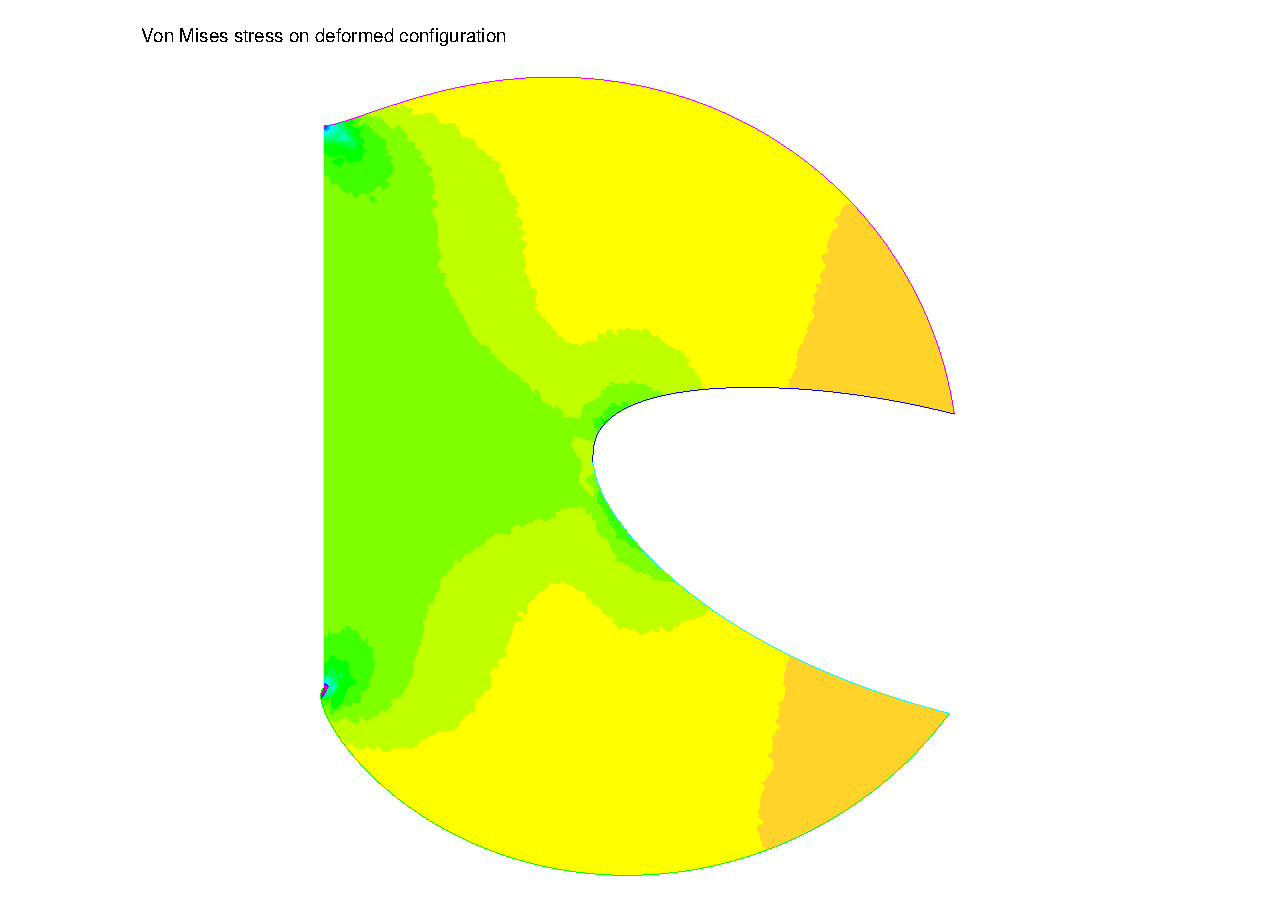
\includegraphics[width=0.7\textwidth]{freefem.eps}
\caption{Converged von Mises stress field superimposed over deformation visualization from FreeFem++ for 33053 elements}
\label{fig:freefem}
\end{figure}

\begin{figure}[!htb]
\centering
\includegraphics[width=0.7\textwidth]{matlab.png}
\caption{Converged von Mises stress field superimposed over deformation visualization from MATLAB for 33053 elements}
\label{fig:matlab}
\end{figure}

\subsection{Largest displacement}

The largest displacement is located at the bottom right tip of the system, as expected. Please see Figure~\ref{fig:matlab}. The point is highlighted on the figure. On the FreeFem++ result it is located at the same place. Please see Figure~\ref{fig:freefem}. 

\clearpage

\bibliographystyle{apalike}
\bibliography{references}

\end{document}